\documentclass[12pt,a4paper]{report}

% ─── Packages ───────────────────────────────────────────────────────────────
\usepackage[a4paper, margin=2.5cm]{geometry}
\usepackage[T1]{fontenc}
\usepackage[utf8]{inputenc}
\usepackage{xcolor}
\usepackage{listings}
\usepackage{titlesec}
\usepackage{tcolorbox}
\usepackage{enumitem}
\usepackage{fancyhdr}
\usepackage{hyperref}
\usepackage{amsmath}
\usepackage{amssymb}
\usepackage{array}
\usepackage{booktabs}
\usepackage{mdframed}
\usepackage{tikz}
\usepackage{setspace}
\usepackage{lmodern}

\tcbuselibrary{most}

\setlength{\headheight}{14pt}

% ─── Colors ─────────────────────────────────────────────────────────────────
\definecolor{primary}{RGB}{41, 98, 255}
\definecolor{accent}{RGB}{0, 184, 148}
\definecolor{codebg}{RGB}{245, 247, 250}
\definecolor{codeframe}{RGB}{200, 210, 230}
\definecolor{keyword}{RGB}{86, 61, 185}
\definecolor{comment}{RGB}{80, 120, 80}
\definecolor{string}{RGB}{180, 50, 50}
\definecolor{titlecolor}{RGB}{20, 30, 70}
\definecolor{chapterbg}{RGB}{41, 98, 255}
\definecolor{notebg}{RGB}{255, 249, 219}
\definecolor{noteframe}{RGB}{210, 170, 0}
\definecolor{tipbg}{RGB}{220, 255, 230}
\definecolor{tipframe}{RGB}{0, 160, 80}
\definecolor{warnbg}{RGB}{255, 230, 230}
\definecolor{warnframe}{RGB}{200, 50, 50}
\definecolor{lightgray}{RGB}{150,150,150}

% ─── Code listing style ──────────────────────────────────────────────────────
\lstdefinestyle{cppstyle}{
    language=C++,
    backgroundcolor=\color{codebg},
    frame=single,
    rulecolor=\color{codeframe},
    basicstyle=\ttfamily\small,
    keywordstyle=\color{keyword}\bfseries,
    commentstyle=\color{comment}\itshape,
    stringstyle=\color{string},
    numbers=left,
    numberstyle=\tiny\color{lightgray},
    numbersep=8pt,
    breaklines=true,
    showstringspaces=false,
    tabsize=4,
    captionpos=b,
    xleftmargin=15pt,
    framexleftmargin=15pt,
    morekeywords={string, nullptr, override, final, auto, noexcept},
}
\lstset{style=cppstyle}

% ─── Chapter style ───────────────────────────────────────────────────────────
\titleformat{\chapter}[display]
  {\normalfont\color{primary}}
  {\large\bfseries\color{primary} Chapter \thechapter}
  {4pt}
  {\Huge\bfseries\color{primary}}
  [\vspace{4pt}{\color{primary}\hrule height 2pt}]

\titlespacing*{\chapter}{0pt}{10pt}{20pt}

% ─── Section style ───────────────────────────────────────────────────────────
\titleformat{\section}{\large\bfseries\color{primary}}{\thesection}{1em}{}
\titleformat{\subsection}{\normalsize\bfseries\color{accent}}{\thesubsection}{1em}{}

% ─── Header / Footer ─────────────────────────────────────────────────────────
\pagestyle{fancy}
\fancyhf{}
\fancyhead[L]{\small\color{lightgray}OOP in C++ -- Prakash Palsaniya}
\fancyhead[R]{\small\color{lightgray}\leftmark}
\fancyfoot[C]{\small\color{lightgray}\thepage}
\renewcommand{\headrulewidth}{0.4pt}

% ─── Custom boxes ────────────────────────────────────────────────────────────
\newtcolorbox{notebox}{
  colback=notebg, colframe=noteframe,
  title=\textbf{Note}, fonttitle=\bfseries,
  left=6pt, right=6pt
}
\newtcolorbox{tipbox}{
  colback=tipbg, colframe=tipframe,
  title=\textbf{Tip}, fonttitle=\bfseries,
  left=6pt, right=6pt
}
\newtcolorbox{warnbox}{
  colback=warnbg, colframe=warnframe,
  title=\textbf{Important}, fonttitle=\bfseries,
  left=6pt, right=6pt
}
\newtcolorbox{conceptbox}[1]{
  colback=codebg, colframe=primary,
  title=\textbf{#1}, fonttitle=\bfseries,
  coltitle=white, attach boxed title to top left={yshift=-2mm, xshift=4mm},
  boxed title style={colback=primary},
  left=6pt, right=6pt, top=10pt
}

% ─── Hyperref setup ──────────────────────────────────────────────────────────
\hypersetup{
    colorlinks=true,
    linkcolor=primary,
    urlcolor=accent,
    pdftitle={OOP in C++ Notes},
    pdfauthor={Prakash Palsaniya},
}

% ─────────────────────────────────────────────────────────────────────────────
\begin{document}

% ── Title Page ───────────────────────────────────────────────────────────────
\begin{titlepage}
\centering
\vspace*{2cm}
{\color{primary}\rule{\textwidth}{3pt}}\\[0.5cm]
{\Huge\bfseries\color{titlecolor} Object-Oriented Programming}\\[0.3cm]
{\huge\bfseries\color{titlecolor} in C++}\\[0.5cm]
{\color{primary}\rule{\textwidth}{3pt}}\\[1.5cm]
{\Large\color{lightgray} Complete Learning Notes}\\[0.3cm]
{\large\color{lightgray} Basics to Advanced --- 10-Day Roadmap}\\[2cm]
\begin{tcolorbox}[colback=primary!10, colframe=primary, width=0.8\textwidth]
\centering
\textbf{Topics Covered:}\\[0.3cm]
Basics \textbullet{} Classes \& Objects \textbullet{} Constructors \& Destructors\\[0.2cm]
Encapsulation \textbullet{} Inheritance \textbullet{} Static Members\\[0.2cm]
Polymorphism \textbullet{} Abstraction \textbullet{} Exception Handling\\[0.2cm]
File Handling \textbullet{} OOP Implementation
\end{tcolorbox}
\vfill
{\large\bfseries Prakash Palsaniya}\\[0.2cm]
{\color{lightgray} GitHub: PrakashPalsaniya/OOPS-C-}\\[0.5cm]
{\color{lightgray}\today}
\end{titlepage}

\tableofcontents
\newpage

% ===========================================================================
% CHAPTER 1 -- BASICS
% ===========================================================================
\chapter{C++ Basics Refresher}

\section{Variables and Data Types}

A \textbf{variable} is a named memory location that stores a value.
Every variable has a \textbf{data type} which determines what kind of value it holds.

\begin{center}
\begin{tabular}{|l|l|l|l|}
\hline
\textbf{Data Type} & \textbf{Size} & \textbf{Example} & \textbf{Use} \\
\hline
\texttt{int}    & 4 bytes  & \texttt{int age = 22;}     & Whole numbers \\
\texttt{float}  & 4 bytes  & \texttt{float x = 3.14;}  & Decimal (low precision) \\
\texttt{double} & 8 bytes  & \texttt{double y = 3.14;} & Decimal (high precision) \\
\texttt{char}   & 1 byte   & \texttt{char c = 'A';}    & Single character \\
\texttt{bool}   & 1 byte   & \texttt{bool b = true;}   & true / false \\
\texttt{string} & variable & \texttt{string s = "hi";} & Text \\
\hline
\end{tabular}
\end{center}

\begin{lstlisting}[caption={Variables and Data Types}]
#include<iostream>
using namespace std;

int main(){
    int    age    = 22;
    float  marks  = 89.5;
    double pi     = 3.14159265;
    char   grade  = 'A';
    bool   passed = true;
    string name   = "Prakash";

    cout << "Name  : " << name   << endl;
    cout << "Age   : " << age    << endl;
    cout << "Marks : " << marks  << endl;
    cout << "Grade : " << grade  << endl;
    return 0;
}
\end{lstlisting}

\section{Pointers and References}

\begin{conceptbox}{Key Concept}
\textbf{Pointer:} A variable that stores the \textit{memory address} of another variable.\\[4pt]
\textbf{Reference:} An \textit{alias} (another name) for an existing variable.
\end{conceptbox}

\begin{lstlisting}[caption={Pointers and References}]
int num = 10;

int *ptr = &num;   // pointer: stores address of num
int &ref = num;    // reference: alias of num

cout << ptr;       // prints address
cout << *ptr;      // dereference: prints 10
*ptr = 50;         // changes num to 50
cout << ref;       // also prints 50 (same variable)
\end{lstlisting}

\begin{notebox}
\texttt{*ptr} means ``value at address stored in ptr'' (dereferencing).\\
\texttt{\&num} means ``address of num''.
\end{notebox}

\section{Functions}

\begin{lstlisting}[caption={Functions -- Call by Value, Reference, Pointer}]
// Call by value -- original NOT changed
void addValue(int x){ x += 10; }

// Call by reference -- original IS changed
void addRef(int &x){ x += 10; }

// Call by pointer -- original IS changed
void addPtr(int *x){ *x += 10; }

int main(){
    int a = 5;
    addValue(a);  cout << a;  // 5  (unchanged)
    addRef(a);    cout << a;  // 15 (changed)
    addPtr(&a);   cout << a;  // 25 (changed)
}
\end{lstlisting}

\section{Stack vs Heap Memory}

\begin{center}
\begin{tabular}{|l|l|l|}
\hline
\textbf{Feature}  & \textbf{Stack}      & \textbf{Heap} \\
\hline
Management        & Automatic           & Manual (new / delete) \\
Speed             & Fast                & Slower \\
Size              & Limited             & Large \\
Lifetime          & Function scope      & Until delete is called \\
Example           & \texttt{int x = 5;} & \texttt{int *p = new int;} \\
\hline
\end{tabular}
\end{center}

\begin{lstlisting}[caption={Stack vs Heap}]
// Stack -- automatic
int a = 10;

// Heap -- manual
int *ptr = new int;   // allocate
*ptr = 99;
delete ptr;           // free
ptr = nullptr;        // good practice

// Heap array
int *arr = new int[5];
delete[] arr;         // use delete[] for arrays
\end{lstlisting}

\begin{warnbox}
Always \texttt{delete} heap memory after use to avoid \textbf{memory leaks}.\\
Use \texttt{delete ptr;} for single variable, \texttt{delete[] arr;} for arrays.
\end{warnbox}

% ===========================================================================
% CHAPTER 2 -- CLASSES & OBJECTS
% ===========================================================================
\chapter{Classes and Objects}

\section{What is a Class?}

A \textbf{class} is a user-defined data type that acts as a \textit{blueprint} for creating objects.
It groups \textbf{data members} (variables) and \textbf{member functions} (methods) together.

\begin{lstlisting}[caption={Basic Class and Object}]
class Student {
  public:
    string name;        // data member
    int    age;
    int    rollNumber;

    void display(){     // member function
        cout << name << " | " << age << endl;
    }
};

int main(){
    Student S1;         // creating an object
    S1.name       = "Prakash";
    S1.age        = 20;
    S1.rollNumber = 101;
    S1.display();
}
\end{lstlisting}

\section{Access Specifiers}

\begin{center}
\begin{tabular}{|l|c|c|c|}
\hline
\textbf{Specifier} & \textbf{Same Class} & \textbf{Child Class} & \textbf{Outside} \\
\hline
\texttt{public}    & Yes & Yes & Yes \\
\texttt{protected} & Yes & Yes & No  \\
\texttt{private}   & Yes & No  & No  \\
\hline
\end{tabular}
\end{center}

\begin{lstlisting}[caption={Access Specifiers}]
class BankAccount {
  private:
    int balance;        // only accessible inside class

  protected:
    string accountType; // accessible in child class too

  public:
    string ownerName;   // accessible from anywhere
    void setBalance(int amount){ balance = amount; }
    void display(){ cout << ownerName << " " << balance; }
};
\end{lstlisting}

\section{The \texttt{this} Pointer}

\texttt{this} is a special pointer inside every class that points to the \textbf{current object}.
It resolves conflicts when parameter names match data member names.

\begin{lstlisting}[caption={this pointer}]
class Student {
    string name;
    int age;
  public:
    Student(string name, int age){
        this->name = name;   // this->name = member
        this->age  = age;    //       name = parameter
    }
    // Returning current object for method chaining
    Student& setName(string name){
        this->name = name;
        return *this;
    }
};
\end{lstlisting}

% ===========================================================================
% CHAPTER 3 -- CONSTRUCTORS & DESTRUCTORS
% ===========================================================================
\chapter{Constructors and Destructors}

\section{What is a Constructor?}

A \textbf{constructor} is a special member function called \textit{automatically} when an object is created.

\begin{itemize}[leftmargin=*]
  \item Same name as the class
  \item No return type (not even void)
  \item Used to initialize data members
\end{itemize}

\section{Types of Constructors}

\subsection{Default Constructor}
Called when no arguments are passed.
\begin{lstlisting}
Customer(){
    name    = "Default";
    balance = 0;
}
Customer A1;   // default constructor called
\end{lstlisting}

\subsection{Parameterized Constructor}
Accepts arguments to initialize with custom values.
\begin{lstlisting}
Customer(string n, int ac, int bal){
    this->name    = n;
    this->ac      = ac;
    this->balance = bal;
}
Customer A1("Prakash", 101, 5000);
\end{lstlisting}

\subsection{Copy Constructor}
Creates a new object as a copy of an existing object.
\begin{lstlisting}
Customer(Customer &obj){
    name    = obj.name;
    balance = obj.balance;
}
Customer A2(A1);   // copy constructor called
\end{lstlisting}

\subsection{Constructor Overloading}
Multiple constructors with different parameters in the same class.
\begin{lstlisting}
Customer(){}                         // 0 args
Customer(string n, int b, int c){}   // 3 args
Customer(string n, int b){}          // 2 args
// Compiler picks correct one based on call
\end{lstlisting}

\subsection{Member Initializer List (Inline Constructor)}
More efficient -- initializes members directly instead of assigning inside body.
\begin{lstlisting}
Customer(string a, int b, int c)
  : name(a), ac(b), balance(c) {}
\end{lstlisting}

\section{Destructor}

A \textbf{destructor} is called automatically when an object goes out of scope or is deleted.

\begin{lstlisting}[caption={Destructor -- free dynamic memory}]
class Customer {
    int *data;
  public:
    Customer(){
        data  = new int;   // allocate on heap
        *data = 10;
        cout << "Constructor called" << endl;
    }
    ~Customer(){           // destructor
        delete data;       // free heap memory
        cout << "Destructor called" << endl;
    }
};
int main(){ Customer A1; }  // destructor auto-called at end
\end{lstlisting}

\begin{notebox}
\textbf{Call Order:} Constructors are called in the order objects are created.
Destructors are called in \textit{reverse} order (LIFO).
\end{notebox}

% ===========================================================================
% CHAPTER 4 -- ENCAPSULATION
% ===========================================================================
\chapter{Encapsulation}

\section{What is Encapsulation?}

\textbf{Encapsulation} is bundling of data and functions into a single unit (class), while restricting direct access to the data from outside.

\begin{conceptbox}{Real-World Analogy}
A \textbf{capsule} hides medicine inside. Similarly, a class hides its private data and exposes only safe public methods.
\end{conceptbox}

\section{Getters and Setters}

\begin{lstlisting}[caption={Encapsulation with getter and setter}]
class Student {
  private:
    string name;
    int    age;
    float  marks;

  public:
    // Setter -- with validation
    void setAge(int age){
        if(age > 0 && age < 100)
            this->age = age;
        else
            cout << "Invalid age!" << endl;
    }
    // Getter
    int getAge(){ return age; }

    void setMarks(float m){
        if(m >= 0 && m <= 100)
            marks = m;
        else
            cout << "Marks must be 0-100!" << endl;
    }
    float getMarks(){ return marks; }
};
\end{lstlisting}

\section{Benefits of Encapsulation}

\begin{itemize}[leftmargin=*]
  \item \textbf{Data hiding:} Private data cannot be accessed directly
  \item \textbf{Validation:} Setters validate data before storing
  \item \textbf{Flexibility:} Internal implementation can change without affecting outside code
  \item \textbf{Security:} Prevents accidental modification of data
\end{itemize}

\begin{tipbox}
Always keep data \texttt{private} and provide \texttt{public} getter/setter methods.
This gives you full control over how data is read and modified.
\end{tipbox}

% ===========================================================================
% CHAPTER 5 -- INHERITANCE
% ===========================================================================
\chapter{Inheritance}

\section{What is Inheritance?}

\textbf{Inheritance} allows a class (child/derived) to acquire properties and behaviors of another class (parent/base). It promotes \textbf{code reuse}.

\begin{lstlisting}[caption={Basic Inheritance}]
// Base class (Parent)
class Animal {
  public:
    string name;
    void eat()  { cout << "Animal is eating" << endl; }
    void sleep(){ cout << "Animal is sleeping" << endl; }
};

// Derived class (Child) -- gets all public members of Animal
class Dog : public Animal {
  public:
    void bark(){ cout << "Dog is barking" << endl; }
};

int main(){
    Dog d;
    d.name = "Bruno";
    d.eat();    // inherited from Animal
    d.bark();   // own method
}
\end{lstlisting}

\section{Access in Inheritance}

\begin{center}
\begin{tabular}{|l|l|l|l|}
\hline
\textbf{Member in Base} & \textbf{public inh.} & \textbf{protected inh.} & \textbf{private inh.} \\
\hline
public    & public    & protected & private \\
protected & protected & protected & private \\
private   & not inherited & not inherited & not inherited \\
\hline
\end{tabular}
\end{center}

% ===========================================================================
% CHAPTER 6 -- TYPES OF INHERITANCE
% ===========================================================================
\chapter{Types of Inheritance}

\section{Single Inheritance}
One child inherits from one parent.
\begin{lstlisting}
class A { public: void showA(){} };
class B : public A {               // B inherits from A
  public: void showB(){}
};
\end{lstlisting}

\section{Multilevel Inheritance}
Chain: A inherits nothing, B inherits A, C inherits B.
\begin{lstlisting}
class Animal { public: void eat(){} };
class Dog    : public Animal { public: void bark(){} };
class BabyDog: public Dog    { public: void weep(){} };

BabyDog bd;
bd.eat();    // from Animal  (Level 1)
bd.bark();   // from Dog     (Level 2)
bd.weep();   // own method   (Level 3)
\end{lstlisting}

\section{Multiple Inheritance}
One child inherits from more than one parent.
\begin{lstlisting}
class Father { public: void property(){} };
class Mother { public: void cooking(){} };

// Child gets both Father's and Mother's methods
class Child : public Father, public Mother {
  public: void study(){}
};
\end{lstlisting}

\begin{warnbox}
\textbf{Diamond Problem:} When two parents share the same function, multiple inheritance causes ambiguity.
Solved using \texttt{virtual} inheritance.
\end{warnbox}

\section{Hierarchical Inheritance}
Multiple children inherit from ONE parent.
\begin{lstlisting}
class Animal { public: void eat(){} };

class Dog : public Animal { public: void bark(){} };
class Cat : public Animal { public: void meow(){} };
class Cow : public Animal { public: void moo(){}  };
\end{lstlisting}

\section{Hybrid Inheritance}
Combination of two or more types of inheritance.
\begin{lstlisting}
// Example: Hierarchical + Multiple
class Vehicle { };
class Car    : public Vehicle { };
class Boat   : public Vehicle { };
class AmphibiousCar : public Car, public Boat { };
\end{lstlisting}

% ===========================================================================
% CHAPTER 7 -- STATIC MEMBERS
% ===========================================================================
\chapter{Static Data Members and Functions}

\section{Static Data Members}

A \textbf{static data member} is \textit{shared across all objects} of a class.
Only \textbf{one copy} exists in memory regardless of how many objects are created.

\begin{lstlisting}[caption={Static data member}]
class Customer {
    string name;
    static int total_customer;   // ONE copy shared by ALL objects
  public:
    Customer(string n, int ac, int bal){
        this->name = n;
        total_customer++;         // increments for every new object
    }
    void display(){
        cout << name << " | Total: " << total_customer << endl;
    }
};

// MUST initialize static member outside class
int Customer::total_customer = 0;

int main(){
    Customer A1("Prakash", 1, 1000);  // total = 1
    Customer A2("Rohit",   2, 2000);  // total = 2
    A1.display();   // prints total = 2
}
\end{lstlisting}

\section{Static Member Functions}

\textbf{Static member functions} can be called \textit{without creating an object}.
They can only access \textit{static} data members.

\begin{lstlisting}[caption={Static member function}]
class Customer {
    static int total;
    static int totalBalance;
  public:
    // Static function -- called using class name, no object needed
    static void showStats(){
        cout << "Total Customers: " << total        << endl;
        cout << "Total Balance  : " << totalBalance << endl;
    }
};

// Call WITHOUT creating any object
Customer::showStats();
\end{lstlisting}

\begin{center}
\begin{tabular}{|l|c|c|}
\hline
\textbf{Feature}              & \textbf{Static Member} & \textbf{Normal Member} \\
\hline
Shared across all objects     & Yes & No \\
Called without object         & Yes (static func.) & No \\
Can access non-static members & No  & Yes \\
\hline
\end{tabular}
\end{center}

% ===========================================================================
% CHAPTER 8 -- POLYMORPHISM
% ===========================================================================
\chapter{Polymorphism}

\section{What is Polymorphism?}

\textbf{Polymorphism} means ``many forms''. The same function name behaves differently based on context.

\begin{center}
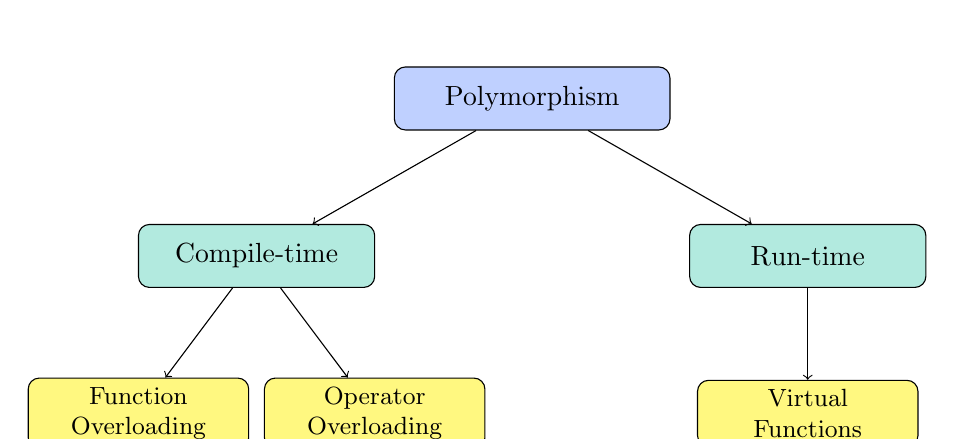
\begin{tikzpicture}[every node/.style={draw, rounded corners, minimum height=0.8cm}]
  \node[fill=primary!30, minimum width=3.5cm] (poly) at (0,0) {Polymorphism};
  \node[fill=accent!30, minimum width=3cm] (ct) at (-3.5,-2) {Compile-time};
  \node[fill=accent!30, minimum width=3cm] (rt) at (3.5,-2) {Run-time};
  \node[fill=yellow!50, minimum width=2.8cm, font=\small, align=center]
    (fo) at (-5,-4) {Function\\Overloading};
  \node[fill=yellow!50, minimum width=2.8cm, font=\small, align=center]
    (oo) at (-2,-4) {Operator\\Overloading};
  \node[fill=yellow!50, minimum width=2.8cm, font=\small, align=center]
    (vf) at (3.5,-4) {Virtual\\Functions};
  \draw[->] (poly) -- (ct);
  \draw[->] (poly) -- (rt);
  \draw[->] (ct) -- (fo);
  \draw[->] (ct) -- (oo);
  \draw[->] (rt) -- (vf);
\end{tikzpicture}
\end{center}

\section{Function Overloading (Compile-time)}
Same function name, different parameters. Compiler picks correct version at compile time.

\begin{lstlisting}[caption={Function Overloading}]
int    add(int a, int b)         { return a + b; }
int    add(int a, int b, int c)  { return a + b + c; }
double add(double a, double b)   { return a + b; }

add(10, 20);      // calls 1st
add(10, 20, 30);  // calls 2nd
add(1.5, 2.5);    // calls 3rd
\end{lstlisting}

\section{Operator Overloading (Compile-time)}
Redefine how operators work for user-defined classes.

\begin{lstlisting}[caption={Operator Overloading -- Complex numbers}]
class Complex {
  public:
    int real, imag;
    Complex(int r, int i): real(r), imag(i){}

    // Overloading + operator
    Complex operator+(Complex c){
        return Complex(real + c.real, imag + c.imag);
    }
    void display(){ cout << real << "+" << imag << "i"; }
};

Complex c1(3,4), c2(1,2);
Complex c3 = c1 + c2;   // uses overloaded +
c3.display();            // prints 4+6i
\end{lstlisting}

\section{Virtual Functions (Runtime Polymorphism)}
The correct version is selected at \textit{runtime} based on the actual object type.

\begin{lstlisting}[caption={Virtual Functions and Runtime Polymorphism}]
class Animal {
  public:
    virtual void sound(){        // virtual keyword
        cout << "Some sound" << endl;
    }
};

class Dog : public Animal {
  public:
    void sound() override {      // override keyword
        cout << "Woof!" << endl;
    }
};

class Cat : public Animal {
  public:
    void sound() override {
        cout << "Meow!" << endl;
    }
};

int main(){
    Animal *ptr;

    Dog d; ptr = &d;
    ptr->sound();   // calls Dog's sound() -- decided at runtime

    Cat c; ptr = &c;
    ptr->sound();   // calls Cat's sound() -- decided at runtime
}
\end{lstlisting}

\begin{tipbox}
Always use \texttt{override} in the child class. If the base function signature does not match,
the compiler will give an error -- helping you catch bugs early.
\end{tipbox}

% ===========================================================================
% CHAPTER 9 -- ABSTRACTION
% ===========================================================================
\chapter{Abstraction}

\section{What is Abstraction?}

\textbf{Abstraction} means showing only \textit{what is necessary} and hiding internal implementation details.

\textbf{Example:} A car driver uses the steering wheel and pedals without knowing the internal engine mechanics.

\section{Abstract Class and Pure Virtual Functions}

A class with at least one \textbf{pure virtual function} is an \textbf{abstract class}.
You \textit{cannot} create objects of an abstract class.

\begin{lstlisting}[caption={Pure Virtual Function and Abstract Class}]
class Shape {                // Abstract class
  public:
    virtual float area()      = 0;   // pure virtual (= 0)
    virtual float perimeter() = 0;   // pure virtual

    void display(){                  // regular function
        cout << "Area     : " << area()      << endl;
        cout << "Perimeter: " << perimeter() << endl;
    }
};

class Circle : public Shape {
    float r;
  public:
    Circle(float r){ this->r = r; }
    float area()      override { return 3.14f * r * r; }
    float perimeter() override { return 2 * 3.14f * r; }
};

class Rectangle : public Shape {
    float l, w;
  public:
    Rectangle(float l, float w): l(l), w(w){}
    float area()      override { return l * w; }
    float perimeter() override { return 2*(l+w); }
};

int main(){
    // Shape s;   ERROR -- cannot instantiate abstract class
    Circle c(7);
    c.display();

    Rectangle r(5,3);
    r.display();
}
\end{lstlisting}

\begin{center}
\begin{tabular}{|l|l|}
\hline
\textbf{Encapsulation} & Hides data using \texttt{private} access \\
\textbf{Abstraction}   & Hides implementation using pure virtual functions \\
\hline
\end{tabular}
\end{center}

% ===========================================================================
% CHAPTER 10 -- EXCEPTION HANDLING
% ===========================================================================
\chapter{Exception Handling}

\section{What is Exception Handling?}

\textbf{Exception handling} manages runtime errors gracefully -- preventing program crashes.

\begin{center}
\begin{tabular}{|l|l|}
\hline
\textbf{Keyword} & \textbf{Purpose} \\
\hline
\texttt{try}   & Block of code that might throw an exception \\
\texttt{throw} & Raises / throws an exception \\
\texttt{catch} & Catches and handles the exception \\
\hline
\end{tabular}
\end{center}

\begin{lstlisting}[caption={Basic Exception Handling}]
int divide(int a, int b){
    if(b == 0)
        throw "Division by zero!";   // throw an exception
    return a / b;
}

int main(){
    try {
        int result = divide(10, 0);  // might throw
        cout << result;
    }
    catch(const char *msg){          // catch the exception
        cout << "Error: " << msg << endl;
    }
    cout << "Program continues..." << endl;
}
\end{lstlisting}

\section{Multiple Catch Blocks}

\begin{lstlisting}[caption={Multiple catch blocks}]
try {
    // code that might throw
}
catch(int e)        { cout << "Int exception: "    << e; }
catch(const char *e){ cout << "String exception: " << e; }
catch(...)          { cout << "Unknown exception caught"; }
\end{lstlisting}

\section{Custom Exception Class}

\begin{lstlisting}[caption={Custom Exception}]
class InvalidAgeException : public exception {
  public:
    const char* what() const noexcept override {
        return "Invalid Age! Must be between 0-120.";
    }
};

void setAge(int age){
    if(age < 0 || age > 120)
        throw InvalidAgeException();
}

int main(){
    try { setAge(-5); }
    catch(InvalidAgeException &e){
        cout << "Caught: " << e.what() << endl;
    }
}
\end{lstlisting}

% ===========================================================================
% CHAPTER 11 -- FILE HANDLING
% ===========================================================================
\chapter{File Handling}

\section{File Handling in C++}

File handling lets us read from and write to files persistently.
Requires \texttt{\#include<fstream>}.

\begin{center}
\begin{tabular}{|l|l|}
\hline
\textbf{Class}    & \textbf{Purpose} \\
\hline
\texttt{ofstream} & Write to file (output) \\
\texttt{ifstream} & Read from file (input) \\
\texttt{fstream}  & Both read and write \\
\hline
\end{tabular}
\end{center}

\begin{lstlisting}[caption={Write to a file}]
#include<fstream>
using namespace std;

int main(){
    ofstream file("data.txt");      // open for writing
    if(file.is_open()){
        file << "Hello, File!" << endl;
        file << "OOP in C++"   << endl;
        file.close();               // always close
    }
}
\end{lstlisting}

\begin{lstlisting}[caption={Read from a file}]
#include<fstream>
using namespace std;

int main(){
    ifstream file("data.txt");      // open for reading
    string line;
    while(getline(file, line)){     // read line by line
        cout << line << endl;
    }
    file.close();
}
\end{lstlisting}

\begin{lstlisting}[caption={File Handling with OOP}]
class Student {
  public:
    string name;
    int    age;

    void saveToFile(){
        ofstream f("student.txt");
        f << name << " " << age;
        f.close();
    }
    void loadFromFile(){
        ifstream f("student.txt");
        f >> name >> age;
        f.close();
    }
    void display(){ cout << name << " " << age << endl; }
};

int main(){
    Student s1; s1.name = "Prakash"; s1.age = 20;
    s1.saveToFile();

    Student s2;
    s2.loadFromFile();
    s2.display();       // prints Prakash 20
}
\end{lstlisting}

% ===========================================================================
% CHAPTER 12 -- OOP IMPLEMENTATION
% ===========================================================================
\chapter{OOP Implementation}

\section{Combining All OOP Concepts}

A well-designed OOP program uses all four pillars together:

\begin{enumerate}[leftmargin=*]
  \item \textbf{Encapsulation} --- keep data private, expose via public methods
  \item \textbf{Abstraction} --- hide implementation, show only interface
  \item \textbf{Inheritance} --- reuse existing code in child classes
  \item \textbf{Polymorphism} --- one interface, many behaviors
\end{enumerate}

\begin{lstlisting}[caption={Mini Bank System -- all OOP concepts}]
#include<iostream>
using namespace std;

// Abstract Base Class (Abstraction)
class Account {
  protected:                    // protected for child access
    string name;
    int    accNo;
    double balance;

  public:
    Account(string n, int a, double b)
      : name(n), accNo(a), balance(b){}

    virtual void display() = 0; // pure virtual (Abstraction)

    // Encapsulated operations with validation
    void deposit(double amt){
        if(amt > 0) balance += amt;
    }
    void withdraw(double amt){
        if(amt > 0 && amt <= balance) balance -= amt;
        else cout << "Insufficient balance!" << endl;
    }
};

// Inheritance -- SavingsAccount extends Account
class SavingsAccount : public Account {
    double interestRate;
  public:
    SavingsAccount(string n, int a, double b, double r)
      : Account(n, a, b), interestRate(r){}

    // Runtime Polymorphism -- overrides display()
    void display() override {
        cout << "Name    : " << name         << endl;
        cout << "Acc No  : " << accNo        << endl;
        cout << "Balance : " << balance      << endl;
        cout << "Rate    : " << interestRate << "%" << endl;
    }
};

int main(){
    Account *acc = new SavingsAccount("Prakash",101,5000,4.5);
    acc->deposit(1000);
    acc->display();    // calls SavingsAccount::display()
    delete acc;
}
\end{lstlisting}

\newpage
\section{OOP Quick Revision Cheat Sheet}

\begin{tcolorbox}[colback=codebg, colframe=primary,
  title=\textbf{OOP in C++ -- Cheat Sheet},
  fonttitle=\bfseries\color{white}, coltitle=white]
\begin{tabular}{ll}
\textbf{class}           & Blueprint for objects \\
\textbf{object}          & Instance of a class \\
\textbf{constructor}     & Auto-called when object is created \\
\textbf{destructor}      & Auto-called when object is destroyed \\
\textbf{this}            & Pointer to the current object \\
\textbf{static}          & Shared across all objects \\
\textbf{private}         & Hidden from outside (Encapsulation) \\
\textbf{protected}       & Accessible in derived class \\
\textbf{virtual}         & Enables runtime polymorphism \\
\textbf{override}        & Explicitly overrides base function \\
\textbf{= 0}             & Pure virtual -- makes class abstract \\
\textbf{try/catch/throw} & Exception handling \\
\textbf{ofstream}        & Write to file \\
\textbf{ifstream}        & Read from file \\
\textbf{new}             & Allocate heap memory \\
\textbf{delete}          & Free heap memory \\
\end{tabular}
\end{tcolorbox}

\vspace{1cm}

\begin{tcolorbox}[colback=tipbg, colframe=tipframe,
  title=\textbf{4 Pillars of OOP}, fonttitle=\bfseries]
\begin{tabular}{lp{9cm}}
\textbf{Encapsulation}  & Wrap data + functions. Keep data \texttt{private}. \\
\textbf{Abstraction}    & Show only essentials. Use pure virtual functions. \\
\textbf{Inheritance}    & Reuse code. Child inherits from parent. \\
\textbf{Polymorphism}   & One interface, many forms. Overloading + Virtual. \\
\end{tabular}
\end{tcolorbox}

\vfill
\begin{center}
{\large\bfseries\color{primary} Keep Learning. Keep Coding.}\\[0.3cm]
{\color{lightgray} github.com/PrakashPalsaniya/OOPS-C-}
\end{center}

\end{document}
